%%
%% This is file `test-algorithms.tex',
%% generated with the docstrip utility.
%%
%% The original source files were:
%%
%% phd.dtx  (with options: `test-algorithms')
%% ----------------------------------------------------------------
%% phd --- short description.
%% E-mail: yannislaz@gmail.com
%% Released under the LaTeX Project Public License v1.3c or later
%% See http://www.latex-project.org/lppl.txt
%% ----------------------------------------------------------------
%% 
^^A \@specialfalse


\newgeometry{top=1.35cm,bottom=2cm,left=2cm}
\clearpage
\cxset{manet/.style={
 chapter opening=anywhere,
 chapter toc=true,
 toc image=false,
 name={},
 numbering=none,
 number font-size=,
 number font-family=,
 number font-weight=,
 number before={\vspace*{-2.5cm}},
 number dot={},
 number after={},
 number position=leftname,
 chapter font-family=,
 chapter font-weight=,
 chapter font-size=,
 chapter before=,
 chapter after={},
 chapter color={black!90},
 number color= teal,
 title beforeskip={},
 title afterskip={},
 title before={\hspace*{-2.47cm}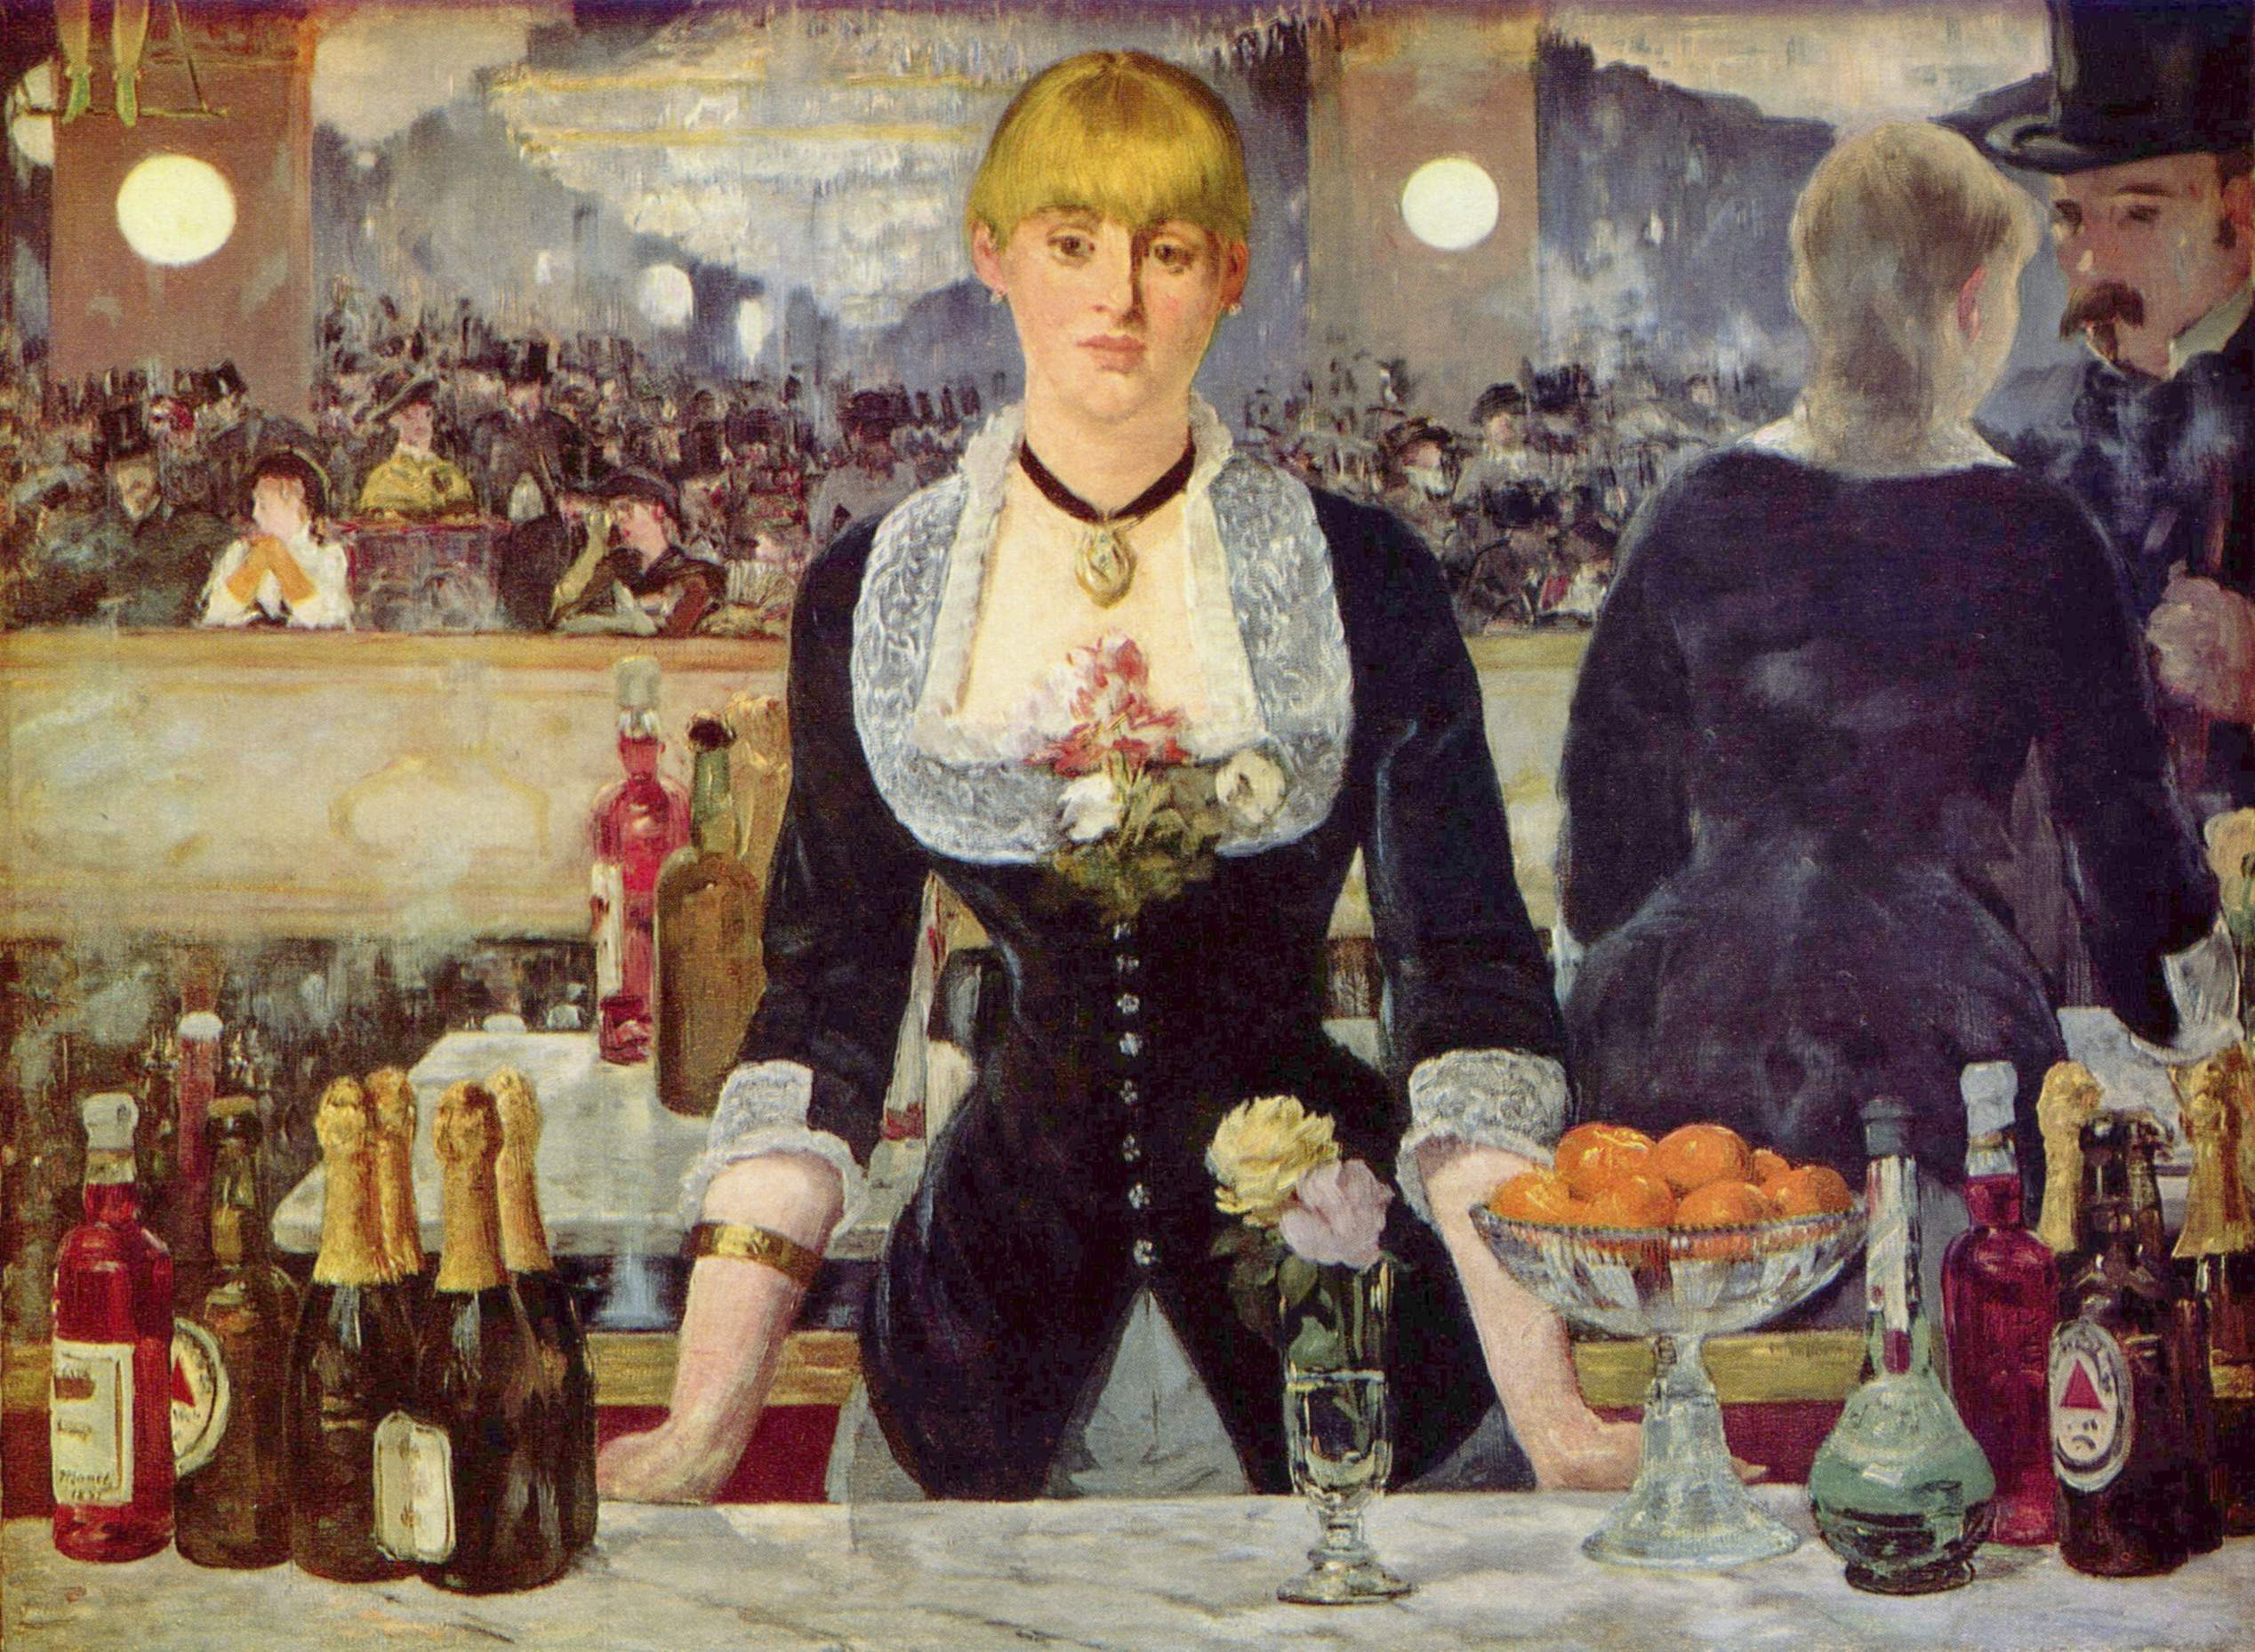
\includegraphics[width=1.27\textwidth]{./chapters/manet}%
    \par\hfill\hfill{\tiny\bfseries Manet's  \textit{The Barmaid.}}\\
    \par
    \vspace*{\baselineskip}
    \par\hfill},
 title after={\hfill\hfill},
 title font-family=\sffamily,
 title font-color= black!80,
 title font-weight=\bfseries,
 title font-size=\LARGE}}
\cxset{manet}



\chapter{A New Approach to Designing \LaTeX\ Classes}
\begin{multicols}{3}
      \leftskip0pt
      \lettrine{I}{psum dolor} sit amet latixeus. \lipsum*[1-2]
      Latinicus porcupinus to fill the line.


This particular code, uses the predefined style \textit{manet}. The only difference we have now defined a helper macro to make it easier for such images to be inserted for similar style chapter openings.
If a full book is to be designed using chapter openings in this fashion more keys and styles could be defined to make it even more easy to enter.
\end{multicols}



\def\topimage#1{\cxset{title before={\hskip-2.3cm\includegraphics[width=1.25\textwidth]{./chapters/#1}\par
\vspace*{\baselineskip}\par}}}




The full code to have the chapter typeset is shown below:


\begin{lstlisting}
\cxset{manet}
\topimage{Alan-MacDonald-Cardinal-Spin-01}

\chapter{ALAN MacDONALD}
\begin{multicols}{3}
      \leftskip0pt
      \lettrine{I}{psum dolor} sit amet latixeus. \lipsum*[1-2]
      Latinicus porcupinus to fill the line.
\end{multicols}
\end{lstlisting}
\lipsum[2]

\loadgeometry{std}




\documentclass{article}
\usepackage{phd}
\begin{document}
\begin{algorithm}[H]
\SetAlgoLined
\KwData{this text}
\KwResult{how to write algorithm with \LaTeX2e }
initialization\;
\While{not at end of this document}{
read current\;
\eIf{understand}{
go to next section\;
current section becomes this one\;
}{
go back to the beginning of current section\;
}
}
\caption{How to write algorithms}
\end{algorithm}
\IncMargin{1em}
\begin{algorithm}
\SetKwData{Left}{left}\SetKwData{This}{this}\SetKwData{Up}{up}
\SetKwFunction{Union}{Union}\SetKwFunction{FindCompress}{FindCompress}
\SetKwInOut{Input}{input}\SetKwInOut{Output}{output}
\Input{A bitmap $Im$ of size $w\times l$}
\Output{A partition of the bitmap}
\BlankLine
\emph{special treatment of the first line}\;
\For{$i\leftarrow 2$ \KwTo $l$}{
\emph{special treatment of the first element of line $i$}\;
\For{$j\leftarrow 2$ \KwTo $w$}{\label{forins}
\Left$\leftarrow$ \FindCompress{$Im[i,j-1]$}\;
\Up$\leftarrow$ \FindCompress{$Im[i-1,]$}\;
\This$\leftarrow$ \FindCompress{$Im[i,j]$}\;
\If(\tcp*[h]{O(\Left,\This)==1}){\Left compatible with \This}{\label{lt}
\lIf{\Left $<$ \This}{\Union{\Left,\This}}\;
\lElse{\Union{\This,\Left}\;}
}
\If(\tcp*[f]{O(\Up,\This)==1}){\Up compatible with \This}{\label{ut}
\lIf{\Up $<$ \This}{\Union{\Up,\This}}\;
\tcp{\This is put under \Up to keep tree as flat as possible}\label{cmt}
\lElse{\Union{\This,\Up}}\tcp*[r]{\This linked to \Up}\label{lelse}
}
}
\lForEach{element $e$ of the line $i$}{\FindCompress{p}}
}
\caption{disjoint decomposition}\label{algo_disjdecomp}
\end{algorithm}\DecMargin{1em}
\end{document}

\endinput
%%
%% End of file `test-algorithms.tex'.
